\section{Related Work}
\subsection{Malware Analysis}
Malware analysis is a critical aspect of cybersecurity, enabling the identification
and mitigation of malicious software threats.
Analysis techniques can be roughly categorized into two classes: static and dynamic.

\subsubsection{Static Analysis}
Static analysis involves examining the structure and content of a suspected malicious file without executing it.
Static analysis are often conducted as a preliminary step to grasp the general characteristics of the malware
before more sophisticated analysis techniques are applied \cite{chakkaravarthy2019survey}.

\textbf{Signature matching} is a common technique that compares the "signature", characteristics of a file
against a database of malware such as VirusTotal \cite{VirusTot28:online}. The characteristics include file size, hash values, and byte sequences.
Although this method has been a staple in malware detection, it is limited by its inability to detect only known malware.

\textbf{Disassemble and decompile} is another static analysis technique
that involves converting the binary code of a malware into a human-readable format.
From the decompiled code, analysts might be able to identify the malware's functionality and behavior as well as finding
interesting strings like URLs, IP addresses, and encryption keys.

\subsection{Dynamic Analysis \cite{10.1145/3329786}}
Dynamic analysis entails examining the behavior of malware by executing it in a controlled environment.
This approach enables analysts to witness the interactions between the malware and the system,
providing insights into its true intentions and capabilities.

\textbf{Function call analysis} is a method that focuses on tracking functions issued by the malware and the parameters
passed to them. One way to archive this is by code injection, in which analyzing code is hooked into
a specific function call and various information is collected and notified when the function is called.
Carsten et al. \cite{willems2007toward} created an automated malware analysis system that injects DLLs within CWSandbox,
letting analysts monitor system calls.

\textbf{Data flow tracking} is another approach that tracks the flow of data through the malware, and data tainting is an established
technique in this area. It involves marking (or "tainting") specific data components and then monitoring
how this tainted data propagates through the system.
Data tainting could be utilized in static analysis, but due to some evasion strategies like encryption and obfuscation
it has endured challenges in practice \cite{alashjee2019dynamic}.
SELECTIVETAINT \cite{chen2021selectivetaint} was invented to address performance overhead issue by employing static binary
rewriting to selectively instrument only instructions related to taint analysis.




\subsection{Berkeley Packet Filter}
StevenとVan \cite{mccanne1993bsd}は1993年に,Unix系のOS上でパケットキャプチャを効率的に行うためのアーキテクチャである
BSD Packet Filterを提案した.以下,Berkeley Packet Filterを「BPF」と表記する. \\
論文発表当時のパケットキャプチャでは,カーネル空間で取得したパケットをすべてユーザー空間にコピーしてからフィルタリングしていて,
これが無駄なオーバーヘッドの原因となっていた.
\cite{mccanne1993bsd}は特殊な32ビット命令で記述されたプログラムを解釈して
フィルタリングを行う疑似マシン (BPF pseudo-machine) を考案し,それをカーネル空間で動作させることでこの問題に対処した.
既存のシステムとの比較では,BPFは最大で20倍程度高速に動作した.
BPFのアーキテクチャの概要を\Fref{img:bpf_old}に示す.

BPFはLinuxカーネルのv2.1.75にてLinux Socket Filterという名前で導入され,\texttt{tcpdump}コマンドの高速化のために使われた.

\subsection{BPFの拡張}
BPFはLinuxカーネルのv3.18にて大幅に改修,拡張が行われ,extended BPFすなわちeBPFと呼ばれるようになった \cite{Linux31836:online}.
拡張された部分は多岐にわたるが,代表的なものを以下に列挙する \cite{learning-ebpf}.
\begin{itemize}
  \item BPF命令セットが32ビットから64ビットに書き直され,実行効率が向上した.
  \item eBPF mapが導入され,ユーザー空間とカーネル空間の間でデータを共有する手段が追加された.
  \item eBPFプログラムが安全に実行できることを検証するeBPF verifierが追加された.
\end{itemize}
\begin{figure}[tp]
  \begin{center}
    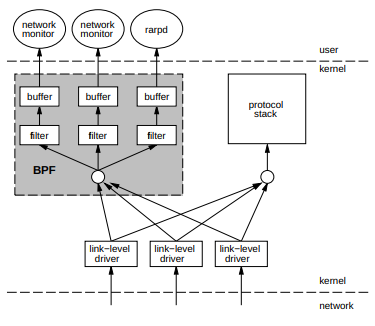
\includegraphics[width=\columnwidth]{./img/bpf_overview.png}
  \end{center}
  \caption{The overview of BPF architecture. It accelerates packet capture
    by performing filtering in the kernel space. \cite{mccanne1993bsd}}
  \label{img:bpf_old}
\end{figure}

また,eBPFがカバーする領域も拡大していった.ネットワークの文脈では,Linuxのネットワークスタックの様々なレイヤー,例えばUnix socket
やネットワークデバイスなどを扱えるようになった.加えてeBPFプログラムはLinuxシステムのパフォーマンストレーシングやセキュリティ向上にも
利用できるようになり,"BPF"という単語は本来の意味である"Berkeley Packet Filter"を失い独立した単語として使われるようになっていった.

便宜上,v3.18における拡張以前のBPFをclassical BPF,あるいはcBPFと呼ぶことがある.

\subsection{eBPFのアーキテクチャ}
eBPFのアーキテクチャの概要を\Fref{img:ebpf-system}に示す.以下,\Fref{img:ebpf-system}を参照しながら重要な
処理フローについて説明する.
\begin{figure}[tp]
  \begin{center}
    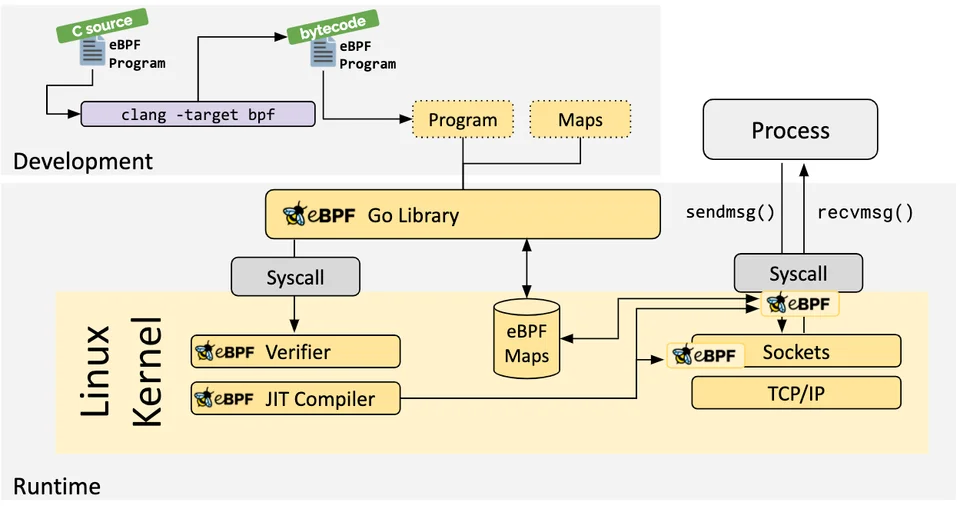
\includegraphics[width=\columnwidth]{./img/ebpf_system.png}
  \end{center}
  \caption{The overview of eBPF architecture. This figure shows how eBPF programs are compiled, verified, and executed.
    \cite{WhatiseB29:online}}
  \label{img:ebpf-system}
\end{figure}

\subsubsection{Event-Driven Architecture}
eBPFはevent-drivenである.カーネル内でのイベントにeBPFプログラムをフックし,
イベントが発生したら所定の処理を行う,という仕組みである.
eBPFプログラムは動的にロードまたは削除することが可能である.

eBPFがフックできるイベントはカーネルのソースコード \footnote{\texttt{include/uapi/linux/bpf.h}} においてProgram Typeとして定義されている.
Program Typeをイベントの種別ごとに分類すると,以下のようなものが挙げられる.
\begin{itemize}
  \item XDP: ネットワークデバイスにパケットが到着したとき,カーネル空間にデータがコピーされる前にパケットを操作するためのイベント.
  \item tracing: カーネル関数の呼び出しやトレースポイントの通過を検知するためのイベント.
  \item LSM: Linux Security Moduleを利用してセキュリティポリシーを適用するためのイベント.
\end{itemize}

このようなイベントが発生したとき,eBPFプログラムはProgram Typeに応じた処理を実行する.
例えばXDPのイベントにフックされているプログラムがパケットをacceptするかdropするかを判断する,といった
処理が可能である.

\subsubsection{eBPF Verifier}
eBPF verifierはバイトコードに変換されたeBPFプログラムを入力とし,そのプログラムがカーネル上で安全に
実行できることを検証するプログラムである.バイトコードは\texttt{bpf()}システムコールで
カーネル上にロードされる (\Fref{img:ebpf-system}の"Syscall") が,verifierによる検証を
通過しない限りプログラムは実行されない.
具体的には,メモリアクセス違反を起こさないことやプログラムが正常に終了すること,
不必要なprivilegeがプログラムに与えられていないことなどが確認されている.

このように,eBPF verifierはeBPFプログラムに制約を課すことで安全性を高めている.
verifierがeBPFにおいて重要な意味を持つことから,verifierのロジックを数学的に検証する
研究 \cite{vishwanathan2023verifying}も行われている.

\subsubsection{JITコンパイル}
verifierを通過したeBPFバイトコードはJITコンパイラによってターゲットのCPU上で直接動作する機械語に変換される.
これにより実行速度が最適化され,ソースコードから直接コンパイルされたカーネルおよびカーネルモジュールと同程度効率的に
動作する.
